\chapter{Ising-Nematic Quantum Critical Point}
\label{chap-ising-nematic}


\abstract{An Ising-nematic quantum phase transition refers to the spontaneous breaking of a fourfold-symmetric Fermi surface (FS) to a twofold symmetric one, brought about by an order parameter whose Landau-Ginzburg action takes the same form as the Ising order parameter quantifying magnetization. Coupling to the itinerant fermionc degrees of freedom of a FS, this order parameter drmataically induces non-Fermi liquid behaviour right at the point where the phase transition takes place. Our aim is to demonstrate how to capture the universal properties that result from the singular interactions between the gapless collective modes, arising from the quantum fluctions of this order parameter, and the soft fluctuations from the quasiparticles residing near the FS. After providing the explicit expressions for one-loop order computations, we also discuss the generic characteristics to be expected from higher-loop calculations.}



\section{Introduction}
\label{sec1}

In this chapter, we focus our attention to a particularly illuminating example: an Ising-nematic order parameter that couples with the quadrupolar distortion of a Fermi surface (FS). At a quantum phase transition, this coupling drives the spontaneous breaking of a fourfold-symmetric FS down to a twofold-symmetric one, and the system crosses through what is known as a non-Fermi liquid (NFL) phase. Our goal in what follows is to show how a controlled quantum field-theoretic analysis --- employing the powerful technique of dimensional regularization --- can be used to determine the low-energy scaling behavior of such NFLs embedded in a generic spatial dimension symbolised by $d$.

For a globally convex FS in momentum space, no single point on the surface is privileged over any other, and the geometry is naturally characterized by two quantities: the dimension $m$ of the FS itself, and its co-dimension $\tilde{d} = d - m$. The virtue of dimensional regularization is that $m$ and $\tilde{d}$ can be varied independently. Roughly speaking, $d$ controls how strongly quantum fluctuations are felt, while $m$ governs how many gapless modes are available. In real physical systems, $d$ and $m$ are of course positive integers (with $d \geq 2$ and $m \geq 1$), but we shall treat them as continuously tunable parameters --- a mathematical artifice that allows us to smoothly approach the physical dimension $d_p$ where the relevant degrees of freedom are strongly coupled. When $d_p$ lies below the upper critical dimension $d_c$, the system flows at low energies toward an interacting NFL; when $d_p > d_c$, a conventional Fermi-liquid (FL) description remains adequate.

Among the NFLs that arise when $d_p < d_c$, there is a qualitative distinction between the cases $m = 1$ and $m > 1$, and the origin of this distinction is worth dwelling on. When $m = 1$, an emergent locality appears in momentum space: observables such as Green's functions, which are local in momentum, can be extracted from small patches of the FS without any reference to its global structure. This locality is what makes controlled NFL descriptions possible in the so-called patch formulation. When $m > 1$, however, this locality is lost. The size of the FS, set by $k_F$, enters the bosonic propagator through the Landau-damping term and qualitatively modifies the scaling behavior. This is a manifestation of UV/IR mixing --- a situation in which low-energy physics is influenced by gapless modes spread across the entire FS, and therefore cannot be captured purely by renormalizing local properties near any given point. In this sense, $k_F$ becomes a ``naked scale'': it resists being absorbed into the local effective description and leaves a permanent imprint on the low-energy theory.

To appreciate why UV/IR mixing is so unusual, it helps to contrast it with the familiar situation in renormalizable relativistic quantum field theories. In QED, for instance, any observable at a momentum $|\boldsymbol{k}_1| \ll \Lambda$ can be expressed entirely in terms of the renormalized mass and charge measured at some other low-energy scale $|\boldsymbol{k}_2| \ll \Lambda$, up to corrections suppressed by powers of $|\boldsymbol{k}_1|/\Lambda$. Long-distance and short-distance physics decouple cleanly. This clean decoupling breaks down in the presence of a FS, because $k_F$ introduces an additional energy scale that satisfies $k_F \gg \Lambda$, and when $m > 1$, low-energy observables near the FS can no longer be expressed solely in terms of effective couplings defined locally in momentum space.

One might hope to evade this complication by working with a critical boson possessing a large number of flavours, or a velocity much greater than the Fermi velocity, since either limit pushes the effects of $k_F$ to very low energies. Yet UV/IR mixing is ultimately unavoidable: as long as the number of flavours and the velocity ratio remain finite, it reasserts itself at sufficiently low energies, either through Landau-damping or through the onset of a superconducting instability. With this motivation in hand, the remainder of the chapter is devoted to a controlled field-theoretic treatment of the NFL arising at the Ising-nematic quantum critical point (QCP) for an $m$-dimensional FS embedded in $d$ spatial dimensions --- one that carefully tracks how interactions and UV/IR mixing together conspire to shape the low-energy scaling behavior.






%%%%%%%%%%%%%%%%%%%%%%%%%%%%%
\section{Model}
\label{model}

%%%%%%%%%%%%%%%%%%%%%%%%%%%
\begin{figure}[t!]
\begin{center}
\subfigure[]{\includegraphics[width =0.45 \textwidth]{2d-FS}}
\hspace{ 1 cm}
\subfigure[]{\includegraphics[width =0.4 \textwidth]{patches.png}} 
\end{center}
\caption{(a) A compact Fermi surface can be divided into two halves, centered 
at $\pm K^*$. In the vicinity of each centre, a separate fermionic field is introduced. 
(b) The compact Fermi surface is approximated by two sheets of non-compact 
Fermi surfaces, with a momentum regularization that suppresses modes lying.}\label{figpatches}
\end{figure}
%%%%%%%%%%%%%%%%

We consider an $m$-dimensional FS coupled to a critical boson 
whose momentum is centered at $\vec{Q} = 0$, embedded in $d_p = m+1$ 
spatial dimensions. One natural way to characterize the resulting NFL is 
through the scaling behavior of the fermionic and bosonic Green's functions. 
For this purpose, it is convenient to anchor the analysis at a particular 
point on the Fermi surface --- call it $K^*$ --- at which the fermionic 
Green's function is defined. At low energies, fermions scatter predominantly 
along the tangential directions of the Fermi surface while interacting with 
the critical boson. In the presence of inversion symmetry, fermions in the vicinity of $K^*$ 
couple most strongly to fermions near the antipodal point $-K^*$, whose 
tangent space coincides with that of $K^*$. With this observation in mind, 
we divide the closed Fermi surface into two halves centered at $K^*$ and 
$-K^*$, and introduce separate fermionic fields $\psi_{+,\lambda}$ and 
$\psi_{-,\lambda}$ to represent the degrees of freedom on each half, as 
illustrated in Fig.~\ref{figpatches}. In this coordinate system, the action 
written in Matsubara-frequency space at temperature $T = 0$ takes the form of
%%%%%%%%%%%%%%%%%
\begin{align}
S & =   \sum_{ \lambda, \, s=\pm}  \int dk \,
\psi_{s, \lambda}^\dagger (k)
\Bigl[ 
 i \,k_0   +  s \, k_{1} +   {\vec L}_{(k)}^2 + H( {\vec L}_{(k)}^2 )  \Bigr] \psi_{s, \lambda}(k) \nonumber \\
 & \qquad +  \frac{1}{2} \int  dk
 \left[ k_0^2 + c_\perp\,k_{1}^2 + c_\parallel {\vec L}_{(k)}^2 \right] \phi(-k) \, \phi(k) \nonumber \\
 &\qquad +   \frac{1}{\sqrt{N}} \sum_{ \lambda, \, s=\pm}   
\int dk \, dq ~  e \,\phi(q) ~  \psi^\dagger_{s, \lambda}(k+q) \, \psi_{s, \lambda}(k) \, .
\label{act0-2}
\end{align}
%%%%%%%%%%%%%%%%%%
Here, $k \equiv \{k_0, \, \boldsymbol{k}\}$ denotes the $(d+1)$-dimensional 
energy-momentum vector, where $\boldsymbol{k}$ comprises the components 
$\{k_j\}$ with $1 \leq j \leq d$, and $dk \equiv {d^{d+1}k}/{(2\pi)^{d+1}}$ 
is the corresponding integration measure. The fields $\psi_{+,\lambda}(k)$ 
and $\psi_{-,\lambda}(k)$ represent fermionic degrees of freedom carrying 
an additional flavor index $\lambda \in \{1, 2, \cdots, N\}$, frequency 
$k_0$, and momenta $\boldsymbol{K}^* + \boldsymbol{k}$ and 
$-\boldsymbol{K}^* + \boldsymbol{k}$, respectively. The component $k_1$ 
denotes the momentum direction perpendicular to the Fermi surface at 
$\pm K^*$, while $\vec{L}_{(k)} \equiv (k_2, k_3, \ldots, k_d)$ collects 
the components running parallel to it. The momentum is rescaled so that 
both the magnitude of the Fermi velocity and the quadratic curvature of 
the Fermi surface at $\pm K^*$ are normalized to unity. Since the FS is locally parabolic in this neighborhood, it is natural to assign 
scaling dimensions of $1$ and $1/2$ to $k_1$ and $\vec{L}_{(k)}$, 
respectively. The function
\begin{align}
H\!\left(\vec{L}_{(k)}^2\right) = \sum_{n=3}^\infty \; 
\sum_{i_1, \ldots, i_n = 2}^{d} c_{i_1, \ldots, i_n} \, 
\frac{k_{i_1} \cdots k_{i_n}}{k_F^{\frac{n-2}{2}}}
\end{align}
collects all cubic and higher-order terms in $\vec{L}_{(k)}$, where $k_F$ 
is a scale of scaling dimension $1$. The integration range of $\vec{L}_{(k)}$ 
in $\int dk$ is set by the extent of the Fermi surface, which is of order 
$\sqrt{k_F}$ in this coordinate system. Finally, the bosonic field $\phi$ 
is a real scalar that couples to the fermions through a Yukawa-like 
interaction. This coupling is obtained by expanding the quadrupolar 
distortion of the Fermi surface around $\pm K^*$ and retaining only the 
leading-order, momentum-independent term~\cite{sachdev_book, lee-review}.

%%%%%%%%%%%%%%%%%%%%%%%%%
\begin{figure}[t!]
\begin{center}
\subfigure{\includegraphics[scale=0.075]{ferm4-scatter.png}}\hspace{2 cm}
\subfigure{\includegraphics[scale=0.1]{fs-tangent.png}} 
\end{center}
\caption{For a FS with dimension $m>1$, any two points on the FS have a commom tangent space which is $(m-1)$-dimensional.\label{fig:patch}}
\end{figure}
%%%%%%%%%%%%%%%%%%%%%%%%%%


Although the action bears a resemblance to the patch theories that have 
been used to describe NFLs for $m = 1$ \cite{Lee-Dalid}, the situation 
for $m > 1$ is qualitatively richer: any two points on the Fermi surface 
share at least $(m-1)$ common tangent vectors. Fig.~\ref{fig:patch} 
illustrates this for the concrete case of a spherical Fermi surface 
embedded in three-dimensional momentum space. Consider two fermions 
carrying momenta $\boldsymbol{k}_{p1}$ and $\boldsymbol{k}_{p2}$, which 
scatter to $\boldsymbol{k}_{p1} + \boldsymbol{q}$ and 
$\boldsymbol{k}_{p2} - \boldsymbol{q}$ by exchanging a boson with 
small momentum $\boldsymbol{q}$. When $m > 1$, the transferred momentum 
$\boldsymbol{q}$ can be tangential to the Fermi surface simultaneously 
at both $\boldsymbol{k}_{p1}$ and $\boldsymbol{k}_{p2}$, which means 
that both fermions remain near the Fermi surface before and after the 
scattering event. As a result, any two fermionic fields on the Fermi 
surface stay strongly coupled in the low-energy limit, even though 
processes involving large momentum transfers are suppressed. This 
stands in sharp contrast to the $m = 1$ case, where such low-energy 
scattering is absent except between antipodal points. Because these
interactions are spread nonlocally across the entire FS in the momentum space, the theory with $m > 1$ is ill-defined in the 
$k_F \rightarrow \infty$ limit, unlike the $m = 1$ case. Put 
differently, the low-energy (IR) observables, such as the fermionic and 
bosonic Green's functions near $k = 0$, cannot be determined until the 
global properties of the Fermi surface --- its size and shape at large 
momenta --- are specified. This is the essence of UV/IR mixing, which in 
the Fermi liquid context is encoded in the Landau parameters, themselves 
nonlocal objects in momentum space.

The scale $k_F$ appearing in $H(\vec{L}_{(k)}^2)$ provides a large-momentum 
cutoff along the directions parallel to the FS. Although these 
higher-order terms are irrelevant by naive power counting, they play an 
essential role in encoding the compactness of the Fermi surface and cannot 
simply be discarded. In principle, retaining this information requires an 
infinite set of independent parameters $\{c_{i_1, \ldots, i_n}\}$, each 
encoding a different aspect of the Fermi surface shape away from $K^*$. 
Rather than working with this full complexity, we instead adopt a simplified 
ultraviolet regularization that captures the essential physics of these 
higher-order terms while remaining tractable analytically. Concretely, we 
replace the kinetic term with a regularized version,
\begin{align}
\label{eqkf}
\sum_{s, \lambda} \int dk \, 
\psi_{s, \lambda}^\dagger (k)
\Bigl[ 
 i\, k_0   +  s  \,k_{d-m} +   {\vec L}_{(k)}^2  \Bigr] \psi_{s, \lambda}(k) \, 
\exp \Big \lbrace \frac {{\vec{L}}_{(k)}^2}  { k_F } \Big \rbrace. 
\end{align}
%%%%%%%%%%%%%
Here the dispersion remains parabolic, but the exponential factor renders 
the FS effectively finite by suppressing the kinematics of 
fermions with $|\vec{L}_{(k)}| > \sqrt{k_F}$, as illustrated in 
Fig.~\ref{figpatches}.

%%%%%%%%%%%%%%%%%%%%
\begin{figure}[t!]
\centering
\subfigure[]{\includegraphics[width  =0.6 \textwidth]{FS-scaling.png}} \hspace{0.4 cm}
\subfigure[]{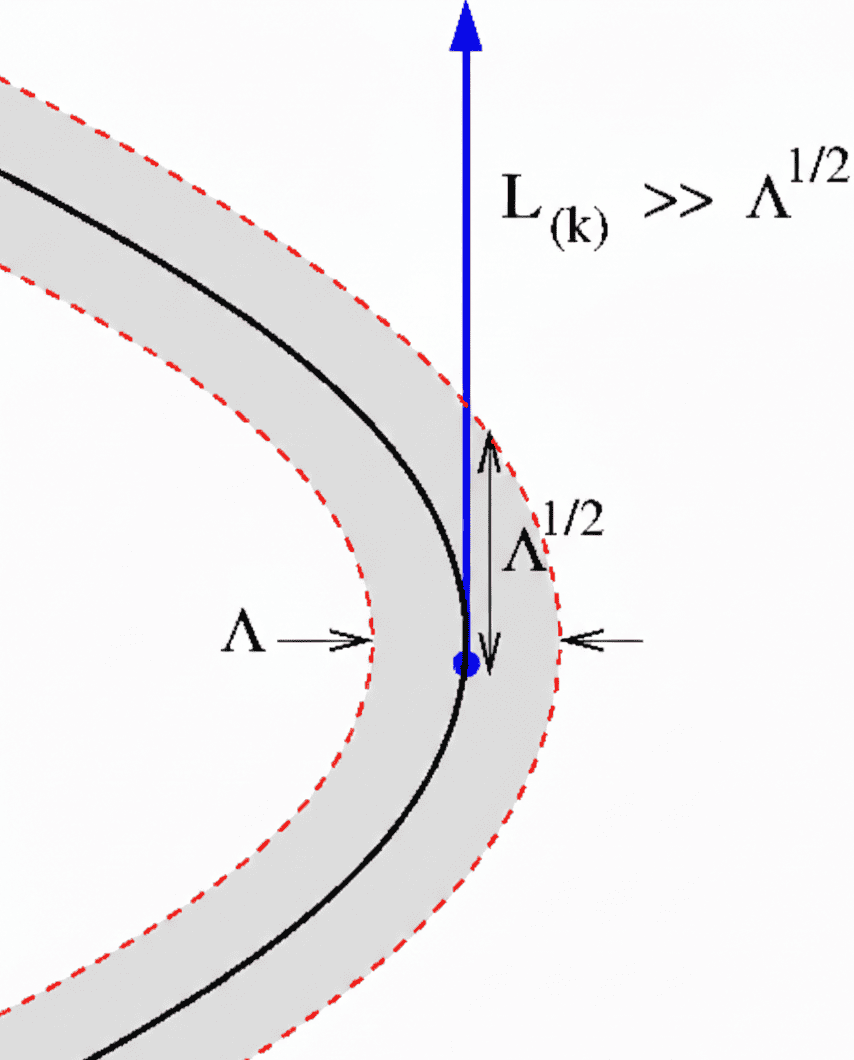
\includegraphics[width  =0.275 \textwidth]{crossover.png}}
\caption{(a) As the high-energy modes away from the FS are integrated 
out, the ratio $k_F/\Lambda$ grows, where $k_F$ denotes the size of the 
FS and $\Lambda$ is the energy cutoff perpendicular to it. 
For $m > 1$, the Green's functions develop singularities in the 
$k_F/\Lambda \rightarrow \infty$ limit, and it is precisely this behavior 
that gives rise to the UV/IR mixing of energy scales. (b) A two-dimensional slice of an $m$-dimensional FS. The 
typical momentum carried by a boson is proportional to 
$\tilde{\alpha}^{1/3}\, \Lambda^{\frac{d-m}{3}} \sim \tilde{e}^{\frac{1}{m+1}} 
\left({k_F}/{\Lambda}\right)^{\frac{m-1}{2(m+1)}} \Lambda^{1/2}$. 
For $m > 1$, this momentum greatly exceeds $\Lambda^{1/2}$ in the 
low-energy limit. Consequently, the momentum transferred by a boson is 
large enough to carry a fermion near the FS well outside the 
thin shell of width $\sim \Lambda$, leading to a suppression of virtual 
particle-hole excitations by powers of $\Lambda/k_F$ for $m > 1$.}\label{fig:FS2}
\end{figure}
%%%%%%%%%%%%%%%%%%

In order to control the Yukawa-like coupling between the fermions and 
bosons, and the strength of the UV/IR mixing, independently of one 
another, we tune both $d$ \cite{Chakravarty,Fit,Torroba} and $m$ 
\cite{senshank,Lee-Dalid,shouvik2}. To maintain the analyticity of the 
theory in momentum space --- which is equivalent to locality in real 
space --- for generic values of $m$, we introduce a two-component 
spinor~\cite{Lee-Dalid,shouvik2},
\begin{align}
\Psi_j^T(k) = \begin{bmatrix} \psi_{+,\lambda}(k) & \quad 
\psi_{-,\lambda}^\dagger(-k) \end{bmatrix},
\end{align}
and use it to formulate an action embedded in a $d$-dimensional momentum 
space, which takes the form of
%%%%%%%%%%%%%%%%%%%%
\begin{align}
\label{eqactphys}
S  &=   \sum_\lambda \int dk \,\bar \Psi_j(k)\,i
\Bigl[ 
{\vec \Gamma} \cdot {\vec K }  + \gamma_{d-m} \, \delta_k \Bigr] \Psi_{j}(k) \,
 e^{ \frac{{{\vec{L}}_{(k)}^2} } {\mu \, {\tilde{k}}_F} }
+ \frac{1}{2} \int  dk \,{\vec{L}}_{(k)}^2\,  \phi(-k) \, \phi(k) 
\nonumber\\ &\quad
 +     \frac{i \, e \, \mu^{x_e/2} }{\sqrt{N}}  \sum_\lambda  
\int dk dq  \,
\phi(q) \, \bar \Psi_{j}(k+q)\,  \gamma_{d-m} \Psi_{j}(k) \,.
%%%%%%%%%%
%\quad \delta_k =  k_{d-m}+ {\vec{L}}_{(k)}^2\,.
\end{align}
%%%%%%%%%%%%%%%%%
Here, $\vec{K} \equiv \{k_0, k_1, \ldots, k_{d-m-1}\}$ collects the 
frequency and the first $(d-m-1)$ components of the $d$-dimensional 
momentum vector, while $\vec{L}_{(k)} \equiv \{k_{d-m+1}, \ldots, k_d\}$ 
and $\delta_k = k_{d-m} + \vec{L}_{(k)}^2$. Within the $d$-dimensional 
momentum space, the components $\{k_1, \ldots, k_{d-m}\}$ and 
$\vec{L}_{(k)}$ represent the $(d-m)$ and $m$ directions perpendicular 
and parallel to the FS, respectively. The vector $\vec{\Gamma} \equiv 
\{\gamma_0, \gamma_1, \ldots, \gamma_{d-m-1}\}$ collects the gamma-matrices 
associated with $\vec{K}$. Since we are interested in co-dimensions 
satisfying $1 \leq d - m \leq 2$, it suffices to work with $2 \times 2$ 
gamma-matrices, for which we take $\gamma_0 = \sigma_y$, 
$\gamma_{d-m} = \sigma_x$, and define $\bar{\Psi} \equiv \Psi^\dagger \gamma_0$.

The leading terms in the non-interacting part of Eq.~\eqref{eqactphys} 
are invariant under the following rescaling transformations, expressed 
in terms of a mass scale $\mu$:
%%%%%%%%%%%%%%%%%%%%%%%%%%%%%%
\begin{align*}
\vec K & = \mu \,{\vec K'} \,, \quad k_{d-m} = \mu \, k_{d-m}' \,,
\quad {\vec{L}}_{(k)} = \sqrt{\mu} \;{\vec{L}}_{(k)}'  \,, \nn
\Psi_j (k) & =  \mu^{ -\,\frac{2 \,d + 4-m}{4}} \,\Psi'_j (k') \,, \quad 
\phi (k) = \mu^{ -\,\frac{2 \,d + 4-m}{4}} \, \phi'(k')\,. 
 \end{align*}
%%%%%%%%%%%%%%%%%%%%%% 
In the quadratic action of the boson, only the term $\vec{L}_{(k)}^2 \, 
\phi^*(k)\phi(k)$ is retained, because $|\vec{K}|^2 + k_{d-m}^2$ is 
irrelevant under the scaling in which each of $\{k_0, k_1, \ldots, 
k_{d-m}\}$ carries dimension $1$ and each of $\{k_{d-m+1}, \ldots, k_d\}$ 
carries dimension $1/2$. Put differently, the bosonic dynamics is so 
strongly dressed by particle-hole excitations that portions of the bare 
kinetic term become unimportant in the infrared. While the $(m+1)$-dimensional 
rotational symmetry of the bosonic action would naively place all of 
$\{k_{d-m}, \ldots, k_d\}$ on equal footing, the coupling to the fermions 
singles out $k_{d-m}$: the bosons that contribute most to fermionic 
scattering around $\pm K^*$ carry momenta satisfying $|\vec{L}_{(k)}| \gg 
k_{d-m}$, and so the dependence on $k_{d-m}$ in the bosonic kinetic term 
can be safely neglected when describing the fermionic dynamics in that 
region. Finally, $c_\parallel$ has been absorbed into a redefinition of 
the field.

The scaling dimension of the Yukawa-like coupling constant $e_0 = e\,\mu^{x_e/2}$ 
is $x_e/2$, where $x_e = 2 + m/2 - d$. By writing $e_0 = e\,\mu^{x_e/2}$, 
where $\mu$ is a mass scale, the coupling $e$ is rendered conveniently 
dimensionless. We further define $\tilde{k}_F = k_F/\mu$ as the 
dimensionless counterpart of $k_F$. The spinor carries an energy dispersion 
with two bands, $E_k = \pm\sqrt{\sum_{j=1}^{d-m-1} k_j^2 + \delta_k^2}$, 
which gives rise to an $m$-dimensional FS embedded in a $d$-dimensional 
momentum space, defined by the $d-m$ conditions $k_i = 0$ for 
$i \in \{1, \ldots, d-m-1\}$ and $k_{d-m} = -\vec{L}_{(k)}^2$.

Apart from $k_F$, which sets the size of the FS, the theory implicitly 
carries a UV cutoff $\Lambda$ for $\vec{K}$ and $k_{d-m}$. It is natural 
to identify $\Lambda = \mu$, which sets the largest energy --- or 
equivalently, the largest momentum perpendicular to the FS --- that 
fermions may carry. If $k_e$ denotes the typical energy scale at which 
one wishes to probe the system, the regime of interest is $k_e \ll 
\Lambda \ll k_F$. We study the RG flows of the two dimensionless 
parameters $e$ and $\tilde{k}_F$, generated by varying $\Lambda$ while 
requiring that low-energy observables remain independent of it. This is 
equivalent to the Wilsonian procedure of coarse-graining, in which 
high-energy modes away from the FS are integrated out at each step. 
Since the zero-energy modes are never integrated out, the ratio 
$k_F/\Lambda$ grows monotonically throughout the coarse-graining 
procedure. We therefore treat $k_F$ as a dimensionful coupling constant 
that flows to infinity in the low-energy limit --- a fact that captures, 
physically, the divergence of the FS size measured in units of the 
thickness of the thin shell surrounding it, as illustrated in 
Fig.~\ref{fig:FS2}(a).


%%%%%%%%%%%%%%%%%%%%%%%%%%%%
\section{Dimensional Regularization}
\label{dr}

%%%%%%%%%%%%%%%%%%%%%%%
\begin{figure}[t!]
\begin{center}
\subfigure[]{\includegraphics[width=0.3 \textwidth]{bos}}
\subfigure[]{\includegraphics[width=0.33 \textwidth]{fermi}} 
\subfigure[]{\includegraphics[width=0.3 \textwidth]{vert}} 
\end{center}
\caption{The one-loop diagrams for the (a) bosonic self-energy, (b) fermionic 
self-energy, and (c) vertex correction. In (a), the gray wiggly curve 
denotes the bare bosonic propagator. The solid arrows represent bare 
fermionic propagators, while the wiggly curves in (b) and (c) denote 
dressed bosonic propagators that incorporate the one-loop self-energy 
shown in (a).}\label{fig1loop}
\end{figure}
%%%%%%%%%%%%%%%%

For a given $m$, we tune $d$ towards the critical dimension, $d_c$, which defines the value of $d$ at which the one-loop quantum corrections diverge logarithmically in $\Lambda$, where $\Lambda \ll k_F$. Clearly, $x_e$ vanishes when $ {\tilde d}_c (m) = 2 + m / {2} $ and, in general, it will turn out that $ {\tilde d}_c \neq d_c$ for $1 <m < 2$.
This mismatch is a sign that $k_F$ enters the low-energy physics in a way that is singular in the large $k_F$ limit, resulting in UV/IR mixing. In order to identify $d_c$, we consider the one-loop quantum corrections.
Since the bare bosonic propagator is independent of $\lbrace k_{0}, \cdots ,k_{d-m} \rbrace $, the loop integrations involving it are ill-defined, unless one resums a series of diagrams that provides a non-trivial dispersion along those directions.
This amounts to rearranging the perturbative expansion such that the one-loop bosonic self-energy [cf. Fig.~\ref{fig1loop}(a)],
$ \Pi_1 (k) = -\, (i\,e)^2\, \mu^{x_e}
\int dq \, \text{Tr}
\left[ \gamma_{d-m} \,G_0 (k+q)\,\gamma_{d-m} \, G_0 (q) \right] $, is included at the `zero'-th order. Our unusual ordering of including Feynman diagrams, which is not organized by the number of loops, is forced upon us by the dynamical structure of the theory. Nevertheless, we adopt a systematic procedure which guarantees that every Feynman diagram is
included once and only once order by order in $\epsilon \equiv d_c - d_p$.




The dressed boson propagator is the one which includes the one-loop self-energy and is expressed as
\begin{align}
\label{eqbabos}
D_1(k) &= \left[ {\vec{L}}_{(k)}^2 - \Pi_1 (k) \right]^{-1} ,\quad
\Pi_1 (k)  = -\,\beta_{d} \, e^2 \, \mu^{x_e}
\frac{ ( \mu \, {\tilde{k}}_F )^{ \frac{m-1}{2}}  \, |\vec K|^{d-m}}{ |\vec{L}_{(k)}| }  \,,
%%%%%%%%%
\nn \beta_d & = \frac{  \Gamma^2 (\frac{d-m+1} {2})} {2^{\frac{2d+m-1}{2}} \, \pi^{\frac{d-1}{2}}  
| \cos \lbrace  \frac{\pi (d-m+1)} {2} \rbrace | \,  \Gamma(\frac{d-m}{2}) \Gamma (d-m+1)}\,,
\end{align}
to the leading order in $k/k_F$, for $|\vec K|^2/|\vec L_{(k)}|^2, ~\delta_k^2/|\vec L_{(k)}|^2 \ll k_F$. The constant $\beta_d$ is finite for $2 \leq d < 3$. Since $D_1(k)$ 
depends on $e$, the higher-loop diagrams are not accompanied by powers 
of $e^2$, but rather by powers of $\tilde{e} = e^{fr}$, where $fr$ is 
a fractional exponent \cite{Lee-Dalid}. The nonanalyticity of the 
exponent in the definition of the effective coupling signals that part 
of the quantum effects of the bosonic self-energy have been incorporated 
nonperturbatively through a resummation of the loop diagrams. It is worth 
emphasizing that $-\Pi_1(k)$ is the celebrated \textit{Landau-damping} 
term, which gives rise to the characteristic $\text{sgn}(k_0)\,|k_0|^{2/3}$ 
dependence of the fermionic self-energy --- a hallmark of NFL behaviour 
across a wide range of quantum critical systems 
\cite{max-isn, max-sdw, Lee-Dalid, ips-uv-ir1, ips-uv-ir2, ips-fflo, ips-2kf, ips-cavity}.
Furthermore, $D_1(k)$ diverges for $m > 1$ in the $k_F \rightarrow \infty$ 
limit. This reflects the fact that Landau-damping grows stronger as the 
FS becomes larger when $m > 1$, since a boson can then decay into 
particle-hole excitations spread across the entire FS. This stands in 
sharp contrast to the $m = 1$ case, where a low-energy boson with a given 
momentum can only decay into particle-hole excitations near isolated patches 
whose tangents are (anti)parallel to its momentum. For $m = 1$ and $m = 2$, $k_F$ drops out of Eq.~\eqref{eqbabos}, 
signaling the absence of UV/IR mixing. We note that Eq.~\eqref{eqbabos} 
is valid only when at least one direction remains tangential to the FS, 
and should therefore not be extended to $m < 1$, where conventional QFT 
methods apply without difficulty. In what follows, we restrict our 
attention to $m > 1$.

The apparent breakdown of the spatial rotational symmetry in the space spanned by the momentum coordinates, 
$\{k_{d-m}, \ldots, k_d\}$, [ cf. Eq.~\eqref{eqbabos}] is an artifact of 
the fact that the expression is valid only for bosons whose momentum is 
nearly tangential to the FS at $\pm K^*$. For a boson propagator with 
a generic momentum, $|\vec{L}_{(k)}|$ in Eq.~\eqref{eqbabos} should 
be replaced by $\sqrt{k_{d-m}^2 + \cdots + k_d^2}$, as required by the 
$(m+1)$-dimensional rotational symmetry. This is because, for any given 
boson momentum $k$, one can always find a point on the FS where $k$ is 
the local tangent. Choosing a coordinate system in which $k_{d-m} = 0$, 
the bosonic self-energy takes exactly the same form as in 
Eq.~\eqref{eqbabos}, and since this holds for any $k$, a generic boson 
propagator must be independent of the direction within the subspace 
spanned by $\{k_{d-m}, \ldots, k_d\}$. In what follows, we work with 
the expression in Eq.~\eqref{eqbabos}, since we are primarily interested 
in the physics near $\pm K^*$ on the FS. The bosons that couple most 
strongly to those two regions carry momenta satisfying $k_{d-m} \ll 
|\vec{L}_{(k)}|$, so that $\sqrt{k_{d-m}^2 + \cdots + k_d^2}$ reduces 
to $|\vec{L}_{(k)}|$ to good approximation. 

Incorporating the dressed bosonic propagator, $D_1$, the one-loop fermionic self-energy, $\Sigma_1 (q)$, needs to be computed, which is shown in Fig.~\ref{fig1loop}(b). An explicit computation leads to~\cite{ips-uv-ir1}
%%%%%%%%%%%%%%%%%%%%%%
\begin{align}
\Sigma_1 (q) &= \frac{(i\,e)^2  \, \mu^{x_e}}  {N} 
\int dk \,\gamma_{d-m} \, G_0 (q-k)\, \gamma_{d-m} \,D_1 (k) \nn
%%%%%%%%%%%%%%%
& = \frac{ -\,i \, e^{2\,(m+1)/3} \, \mu^{ x_e \, (m+1)/3} \, \vec \Gamma \cdot \vec Q    }
{ 6\, N \,   \pi^{(m-1)/2}
(4 \pi)^{\frac{d-m}{2}} \,2^{m-1} \,  | \sin \lbrace (m+1) \pi/3 \rbrace |\, 
 \beta_{d}^{(2-m)/3}  \,( \mu \, {\tilde{k}}_F )^{(m-1)(2-m)/6} }  \nn
& \; \quad \times \frac{  \Gamma ( \frac{3-  (m+1)(d-m) }{6}) \, 
\Gamma (  \frac{d-m-2 \beta}{2}) \,  \Gamma (  \frac{d-m+1}{2})  } 
{  \Gamma{(m/2)} \, \Gamma(\beta) \,  \Gamma ( d-m -  \beta + \frac{1}{2})
\, (\vec Q ^2)^{  \frac{3-  (m+1)(d-m) }{6}} } \,,
\label{eqsigma1}
\end{align} 
where  $\beta \equiv  {(d-m) \,(2-m)}/ {6}$. $\Sigma_1 (q)$ shows a logarithmic divergence
in the IR-scale $\Lambda$ at $ d_c(m) = m + {3}/(m+1) $. The value of $ d_c(m) $ is clearly smaller than ${\tilde d}_c$ within the range $1 <m<2$.
Setting $d=d_c(m) - \epsilon$, the divergence $\sim \ln \Lambda $
corresponds to the divergence captured by the pole, $1/\epsilon$, when translated into the language of dimensional regularization. This can be seen by rewriting the fermionic self-energy as
%%%%%%%%%%%
\begin{align}
\Sigma_1 (q) &= 
\left [ -\, \frac{e^{2 \,(m+1 ) /3}  } {{\tilde{k}}_F ^{ \frac{(m-1) (2-m)} {6}} \,N} 
\frac{u_1}{\epsilon}  + \text{ finite terms}
\right ] \left(i \, \vec \Gamma \cdot \vec Q \right ) ,\nonumber \\
%%%%%%%%%%%%
u_1 &= \frac{ \left( \pi/\beta_d \right)^{\frac{2-m}{2}} }
{ (4 \pi)^{\frac{3}{2(m+1)}} 2^{m-1}  
\left | \sin \Big( \frac{(m+1) \pi} {3} \Big) \right |  }
\, \frac{  \Gamma\Big (  \frac{m+4}{2(m+1)} \Big )  } 
{  \Gamma \big (\frac{m}{2} \big)\, \Gamma \Big (\frac{2-m}{2(m+1)}\Big )
 \, \Gamma \Big(  \frac{2m+5}{2(m+1)} \Big) }\,,
\end{align}
keeping terms upto the leading order in $q/k_F$.
%%%%%%%%%%%%%%%%%%%%%%
The one-loop vertex correction is shown in the Feynman diagram of Fig.~\ref{fig1loop}(c). It vanishes identically, which can be traced back to the existence o aa Ward identity \cite{Lee-Dalid}. The key advantage of our formalism is that we can tune the value if $ m$ from $ 1$ to $ 2 $ with the help of the expansion-parameter $\epsilon$, which remains small as required. Thus, we achieve a controlled perturbative expansion through $\epsilon $, as long as we remain within $1 \leq m \leq 2 $. We would like to emphasize that we are tuning the two dimenionalities, namely, $m$ and $d$, independently, which of course must obey the constraint $m<d$ to make any physical sense. This allows us to tune $d$ such that $\epsilon =  d_c(m) - d $ is perturbatively small for a given $m$.


Eq.~\eqref{eqactphys} is taken to be the \textit{physical action}, 
defined at an energy scale $\mu \sim \Lambda$, and consists of the 
fundamental Lagrangian expressed in terms of non-divergent quantities. 
However, loop integrals generically produce divergent contributions, 
and to handle these we employ renormalization via dimensional 
regularization. The UV-divergent terms are those that arise in the 
$\epsilon \rightarrow 0$ limit. To systematically control these 
divergences, we work within the minimal subtraction ($\mathrm{MS}$) 
renormalization scheme \cite{thooft, weinberg}, in which the divergent 
parts of loop contributions are cancelled by adding appropriate 
counterterms. More precisely, we adopt the modified minimal subtraction 
($\overline{\mathrm{MS}}$) scheme, wherein one absorbs not only the 
strictly divergent pole but also the universal finite term proportional 
to $\epsilon^0$ that invariably accompanies the $1/\epsilon$ pole into 
the corresponding counterterm. 


The counterterm action, $S_{CT}$, which is designed to absorb all singular 
contributions, is constructed by introducing counterterm factors as power 
series $A_{\zeta} = \sum_{n=1}^\infty Z_{\zeta,n}/\epsilon^n$ with 
$\zeta \in [1,4]$, chosen so as to cancel the divergent $1/\epsilon^n$ 
contributions from the Feynman diagrams. It takes the form of
%%%%%%%%%%%%%%%%%%%%
\begin{align}
\label{actcount}
S_{CT}  &=   \sum_\lambda \int dk \,\bar \Psi_\lambda (k)\, i
\Bigl[ A_1 \, {\vec \Gamma} \cdot {\vec K } 
+ A_2 \, \gamma_{d-m} \, \delta_k \Bigr] \Psi_\lambda (k) \,
 e^{ \frac{{{\vec{L}}_{(k)}^2} } {\mu \, {\tilde{k}}_F} }
%%%%%%%
\nn & \quad + \frac{A_3}{2} \int  dk \,{\vec{L}}_{(k)}^2\,  \phi(-k) \, \phi(k) 
\nonumber\\ &\quad
 +   \frac{i \, e \, \mu^{x_e/2} }{\sqrt{N}}  \sum_\lambda  
\int dk dq  \,A_4 \,\phi(q) \, \bar \Psi_\lambda (k+q)\,  \gamma_{d-m} \Psi_\lambda (k) \,.
\end{align}
%%%%%%%%%%%%%%%%%
Due to the $(d-1)$-dimensional rotational invariance in the space 
perpendicular to the FS, each term in $\vec{\Gamma} \cdot \vec{K}$ is 
renormalized in the same way. A Ward identity enforces $A_4 = A_3$ 
\cite{Lee-Dalid}. Subtracting $S_{CT}$ from the so-called \textit{bare} 
action $S_{\text{bare}}$, we obtain the renormalized action, which 
serves as the \textit{physical} effective action of the theory, 
rewritten entirely in terms of non-divergent quantum parameters. Here,
%%%%%%%%%%%%%%%%%%%%%%%%
\begin{align}
\label{act7}
S_{\text{bare}} & =   \sum_\lambda \int d k_B
\, \bar \Psi_{B \lambda }(k_B) \, i
\Bigl[  \vec \Gamma \cdot \vec K_B +  \gamma_{d-m} \delta_{k_B}  \Bigr] 
\Psi_{B \lambda }(k_B) \, \exp \Big \lbrace \frac {{\vec{L}}_{(k),B}^2}  {  k_{F,B} } \Big \rbrace
\nonumber\\
&\quad +\frac{1}{2} \int  d k_B \,
 {\vec{L}}_{(k)}^2\,  \phi_B(-k_B) \, \phi_B(k_B) \nonumber \\
 & \quad +     \frac{i \, e_B }{\sqrt{N}}  \sum_\lambda  
\int d k_B \, d q_B \,\phi_B(q_B) \, \bar \Psi_{B \lambda }(k_B+q_B) 
\, \gamma_{d-m} \Psi_{B \lambda }(k_B) \, ,
\end{align}
%%%%%%%%%%%%
consisting of the \textit{bare quantities}, each labelled with the subscript ``$B$''.
While the bare parameters may be divergent, the physical observables 
are identified with the renormalized coupling constants, which evolve 
as functions of the logarithm of the floating energy scale 
$\mu = \mu_0\,e^{-l}$. We now relate the bare quantities to their 
renormalized counterparts --- written without the superscript ``$B$'' 
--- via the multiplicative $Z_\zeta$-factors, such that
$S_{\text{bare}}  =  S + S_{CT}$ and $ Z_{\zeta}  =  1 + A_{\zeta}$.
%%%%%%%%%%%%%%%%%%%
Here,
\begin{align*}
& \vec K = \frac{Z_2}{Z_1}\, \vec K_B \, , \quad k_{d-m} = k_{B, d-m} \, , 
\; {\vec{L}}_{(k)} = {\vec{L}}_{(k), B} \,, 
\; \Psi(k)  =  \frac{\Psi_B(k_B) } {\sqrt{ Z_\Psi}}\,, 
\;   k_F =\mu \, {\tilde{k}}_F\,,
%%%%%%%%%%
\nn & \phi(k) = \frac{ \phi_B(k_B)}  { \sqrt{Z_\phi} }\,, \;
e_B  =  \frac{1} {\sqrt{Z_3}} 
\left( \frac{Z_2}{Z_1} \right)^{\frac{d-m} {2} } \mu^{ \frac{x_e} {2} }  e\,,
%%%%%%%%%%
\nn & Z_\Psi =  Z_2 \left( \frac{Z_2}{Z_1} \right)^{d-m}, \;
Z_\phi = Z_3 \left( \frac{Z_2}{Z_1} \right)^{d-m}.
\end{align*}
%%%%%%%%%%%%%%
Restricting to the one-loop order, we have $Z_\zeta = 1 + \frac{Z_{\zeta,1}}{\epsilon}$, with
\begin{align}
 Z_{1,1} = - \,e^{ 2\, (m+1 ) /3}  \, u_1  /\big [ {\tilde{k}}_F^{ \frac{(m-1)\, (2-m)} {6}} \,N  \big ] 
\text{ and } Z_{2,1}  = Z_{3,1} = Z_{4,1} =  0 \,.
\end{align}


In the language of Renormalization Group (RG) transformations, the beta-function of a coupling-constant $g$ is defined as $\beta_g = \partial_{\ln \mu} g = \mu\, \partial_\mu g \equiv \partial_l g$. As we integrate out energy-shells, $\beta_g$ is the function that determines the flow of $g$ with $\ln \mu$. At one-loop level, for the two coupling-constants, $\tilde k_F$ and $e$, the beta-functions take the forms of
%%%%%%%%%%%%%%%%%%%%%%
\begin{align}
& \beta_{\tilde k_F}  = -\, \tilde k_F \,, \quad
\beta_e = 
 - \left[ \frac{\epsilon}{2} + \frac{(m-1) \, (2-m)}{4 \, (m+1)} \right]  e 
+ \frac{ u_1 \, {\tilde e} }{2 \, N} \, e \,,\nn 
%%%%%%%%%%%%%%%%%%%
& {\tilde e} \equiv \frac{e^{ 2 (m+1 ) /3}  } 
{{\tilde{k}}_F ^{ \frac{(m-1) \,(2-m)} {6}}} \,,\quad
z = 1 - \frac{\partial} {\partial {\ln \mu}} \left(\frac{Z_2} {Z_1}\right) ,\quad
\eta_\psi = \frac{\mu}{2} \, \frac{\partial {Z_\psi}} {\partial {\mu}} \,, \quad
\eta_\phi = \frac{\mu}{2} \, \frac{\partial {Z_\phi}} {\partial {\mu}}\,.
\label{eq:be}
\end{align}
%%%%
Here, $z$ is the dynamical critical exponent and $\eta_\psi$ ($\eta_\phi$) incorporates the anomalous dimension for the fermions (bosons). The quantity $\tilde{k}_F$ increases under the RG flow because the size 
of the FS, measured in units of $\mu$, grows at low energies. The first 
term in $\beta_e$ indicates that $e$ remains strictly relevant at 
$d = d_c(m)$ for $1 < m < 2$, as reflected by $x_e > 0$ and 
$\tilde{d}_c > d_c$. Intriguingly, the form of the loop correction --- 
the second term --- reveals that higher-order corrections are controlled 
not by $e$ itself, but by an effective coupling $\tilde{e}$, which is 
responsible for the $e^{fr}$ powers that accompany them, as discussed 
earlier. The beta-function for $\tilde{e}$, which no longer contains 
$\tilde{k}_F$, is given by
%%%%%%%%%%%%%%%%%%%
\begin{align}
\label{bstable}
 \beta_{\tilde e}   = -\, \frac{(m+1)\, \epsilon}{3} \, {\tilde e} 
+ \frac{ (m+1)\,  u_1} {3N} \, {\tilde e}^2 + \mathcal{O}({\tilde e}^3) \,.
\end{align}
%%%%%%%%%%%
From this, we see that $\tilde{e}$ flows to an IR-stable fixed point at 
$\tilde{e}^* = N\epsilon/u_1 + \mathcal{O}(\epsilon^2)$. For small 
$\epsilon$, this interacting fixed point is perturbatively accessible, 
despite the fact that the scaling dimension $x_e$ of the bare coupling 
$e$ remains positive in the $\epsilon \rightarrow 0$ limit for 
$1 < m < 2$. Although $e$ grows at low energies, this growth is 
compensated by the Landau damping, which also strengthens as the 
effective size of the FS increases. It is the competition between the 
interaction and the Landau damping that renders the effective coupling 
marginal at the true critical dimension $d_c$, which does not coincide 
with $\tilde{d}_c$ for $1 < m < 2$. We also observe that $k_F$ drops 
out of the effective coupling not only for $m = 1$ but also for $m = 2$. 
In the latter case, the $k_F$ dependence arising from the Landau damping 
is precisely cancelled by the $k_F$ dependence from the phase space of 
intermediate states in Fig.~\ref{fig1loop}(b). Nevertheless, UV/IR 
mixing persists for all $m > 1$, since the Landau damping diverges in 
the large-$k_F$ limit. Finally, the fixed-point values of $\{z, \eta_\psi, \eta_\phi\}$ 
evaluate at one-loop order to $z^* = 3/[3 - (m+1)\,\epsilon]$ and 
$\eta_\psi^* = \eta_\phi^* = -\epsilon/2$. It is remarkable that these 
exponents turn out to be insensitive to the details of the FS --- such 
as $\beta_d$ --- despite the fact that patch scaling is violated by 
$k_F$. This vindicates our use of the exponential cutoff scheme in 
Eq.~\eqref{eqkf}, which captures the compactness of the FS in a minimal 
way without requiring knowledge of its precise shape. The finite anomalous 
dimensions arise from a dynamical balance between the two strongly 
relevant couplings, $e$ and $k_F$ --- a mechanism that is qualitatively 
opposite to cases where finite anomalous dimensions emerge from a balance 
between two \textit{irrelevant couplings} \cite{shouvik2}.




%%%%%%%%%
\section{Renormalization-Group equations}
\label{secrg}

A renormalized Green's function, $G^{({n_\psi} ,{n_\psi} , {n_\phi} )}$, defined by the expectation value,
$$ \Bigl< \phi( k^{1} ) \cdots \phi(k^{{n_\phi} })\,
\Psi( k^{{n_\phi} +1} ) \cdots \Psi(k^{{n_\phi}+n_\psi })\,
 \bar \Psi( k^{n_{\phi}+n_\psi+1} )  \cdots \bar \Psi(k^{n_\phi+2 \,n_\psi} ) \Bigr> $$
 %%%%%%%%%%%%%%%%%
$ = G^{({n_\psi} ,{n_\psi} , {n_\phi} )}( \{ k^\alpha \}; \tilde e, \tilde k_F , \mu )$
$\delta^{d+1} \left( \sum_{\alpha =1}^{{n_\phi+n_\psi} } k^\alpha 
- \sum_{ \alpha^\prime ={n_\phi} + n_\psi +1}^{2 {n_\psi} + {n_\phi}} k^{ \alpha^\prime} \right)$,
is the one which satisfies the RG equation. This is expressed as
%%&&%%%%%%%%%%%%%
\begin{align}
& \Bigg [
- \sum_{ \alpha=1}^{2 \,{n_\psi}  + {n_\phi} } \left(
z \, \vec K^\alpha \cdot \nabla_{K^\alpha}
+ k^{\alpha^\prime}_{d-m} \, \partial_{k^{\alpha^\prime}_{d-m}}
+ \frac{ \vec{L}_{(k^\alpha)} } {2}   \cdot  \nabla_{{L}_{(k^\alpha)}}
\right)  
+ \beta_{\tilde k_F}  \partial_{\tilde k_F}
+ \beta_{\tilde e}  \partial_{\tilde e}
%% %%%%%%%%%%%%%%%%%
\nn & \quad + 2  \, {n_\psi}  \left ( -  \frac{2 \, d_c - 2 \, \epsilon + 4 -m }{4} +  \eta_\psi \right)   
%%%%%%%%%%%%
 +  {n_\phi} \left ( -  \frac{2 \, d_c - 2 \, \epsilon +4 -m }{4} +  \eta_\phi \right) 
+  d_c - \epsilon \nn & \quad
%%%%%%%%%%%%%
 + 1 - \frac{m}{2}  + (d_c - \epsilon - m)\, (z-1)
\Bigg ]
\, G^{({n_\psi} , {n_\psi}  ,{n_\phi})}(\{ k_i \}; {\tilde e}, \tilde k_F , \mu ) 
= 0 \,.
\label{RGeq}
\end{align}
%%%%%%%%%%%%%%%%%
A generic $G^{({n_\psi} ,{n_\psi} , {n_\phi} )}$ contains both fermionc and bosonic fields. In particular, we are interested in the two-point functions for the bosons and the fermions because they contain the information of the generic scaling-form at the IR fixed point. These are:
\begin{align}
\label{Dk0}
G^{(0,0,2)} &=  \frac{1}{ \left (  \vec{L}_{(k)}^2 \right )^{ 2 \Delta_\phi } } \,
f_F \left( 
\frac{| \vec K |^{1/z^*} }{  \vec{L}_{(k)}^2 } ,  \frac{k_{d-m} }{k_F} ,  
\frac{  \vec{L}_{(k)}^2 } {k_F}
\right),   \nn
G^{(1,1,0)} & =   \frac{1}{ | \delta_k |^{ 2 \Delta_\psi} } \,
f_B \left( \frac{ | \vec K |^{1/z^*} }{\delta_k} , \frac{\delta_k }{k_F} ,  \frac{  \vec{L}_{(k)}^2 } {k_F}
 \right) , 
\end{align}
where 
$2 \,\Delta_\phi = 1 - (z^*-1) \left (\frac{3}{m+1}-\epsilon \right) - 2 \,\eta^*_\phi = 1+O(\epsilon^2)$ and
$2\, \Delta_\psi = 1 - (z^*-1) \left (\frac{3}{m+1}-\epsilon \right) - 2 \,\eta^*_\psi = 1+O(\epsilon^2)$.
From the expressions at one-loop order, we infer the universal scaling-forms to be
%%%%%%%%%%%%%%%%%%%%%%%%%%%%
\begin{align}
& f_B( X,Y,Z)  =  \left[1 + \beta_d \, {\tilde e}^{\frac{3}{m+1}}
X^{\frac{3}{m+1} }
Z^{-\frac{3(m-1)}{2(m+1)}}
\right]^{-1}, \nn &
f_F( X,Y,Z)  =  -i \left[ C \, ( {\vec  \Gamma} \cdot \hat {\vec K} ) \, X   + \gamma_{d-m} \right]^{-1} ,
%%%%%%%
C = \mu^{ \frac {m+1}{3} \epsilon  } \left [
1 - \frac{(m+1) \, \gamma \, \epsilon } {6}
\right ],
\end{align}
in the limit $ Y, Z \rightarrow 0$ with $X$ held fixed. 
The expressions show that $f_D$ has a singular dependence on $ Z $ 
in the $ Z\rightarrow 0$ limit. We notice that the sliding symmetry being absent for the momentum coordinates of $\delta_k$ and $\vec L_{(k)}$,
the fermionic Green's function's dependence on $\delta_k$ and $\vec L_{(k)}$ is distinct in general.

%%%%%%%%%%%%%%%
\section{Physical relevance of the expansion-parameter $\epsilon $}
\label{dimexp}

The motivation for employing dimensional regularization and, ultimately, 
the small-$\epsilon$ expansion is to shed light on the stark difference 
in the characteristics of NFLs with $d_p = 2$ and $d_p = 3$. Since the 
former has an $m = 1$ FS, $k_F$ plays no role in the low-energy scaling. 
By contrast, $k_F$ enters as an important scale for $d_p = 3$ NFLs 
precisely due to UV/IR mixing. We now examine how this transition occurs 
in a systematic way by tuning $d$ and $m$ continuously. Although systems 
with non-integer dimensions are unphysical in their own right, they 
provide valuable insight into how $d$ and $m$ each contribute to the 
distinct properties of metals in actual physical dimensions.

For $d_p = 3$, one has $m = 2$, and $k_F$ is seen to drop out of the 
expression for $\tilde{e}$. Nevertheless, the intrinsic UV/IR mixing 
still manifests itself in the dispersion relations of the fermion and 
boson, which go as $k_0 \sim k_x + \vec{L}_{(k)}^2$ and 
$k_0 \sim \vec{L}_{(k)}^3$, respectively, up to small corrections. 
These two fields can have different effective dynamical critical exponents 
at the scale-invariant fixed point, with the mismatch compensated by 
$k_F$. Our analysis therefore yields the correct scaling behavior, 
consistent simultaneously for both bosons and fermions, by incorporating 
the dimensional parameter $k_F$ in an appropriate way. This stands in 
contrast to the $m = 1$ case, where the dispersions of bosons and 
fermions obey the same scaling behavior \cite{Lee-Dalid}. UV/IR mixing 
also plays an important role in suppressing higher-loop quantum 
corrections for $m > 1$, a point we turn to in the next section.



%%%%%%%%%%%%%
\section{Higher-Loop Diagrams And Expansion Parameter}
\label{secexp}

In Ref.~\cite{Lee-Dalid}, the $d_p = 2$ case was treated, where the 
two- and three-loop Feynman diagrams were shown to be suppressed by positive 
powers of $\tilde{e}$, with $\tilde{e} = \mathcal{O}(\epsilon)$. A 
general argument also exists outlining why higher-loop diagrams are 
systematically suppressed by successively higher powers of $\tilde{e}$. 
Our systematic expansion in $\epsilon$ is distinct from an expansion in 
powers of $1/N$, and does not suffer from the proliferation of planar 
diagrams that afflicts the $1/N$ expansion \cite{SSLee-largeN, max-sdw}. 
The introduction of extra codimensions mathematically suppresses the 
density of states at low energies, thereby reducing quantum fluctuations. 
This results in a weaker infrared singularity, which in turn permits a 
controlled expansion for sufficiently small $\epsilon$. We have generalized the treatment of Ref.~\cite{Lee-Dalid} to $d_p > 2$, 
where consequently $m > 1$. While the suppression of higher-loop diagrams 
by positive powers of $\tilde{e}$ persists unchanged for $m > 1$, a 
qualitatively new feature emerges: the explicit appearance of an 
additional energy-scale in the form of $k_F$.


To make an estimate of the magnitude of higher-loop corrections, we first discuss 
an interplay between $k_F$ and $\Lambda$ that plays an important role 
for $m > 1$. Let $k = \{\mathbf{K}, k_{d-m}, \vec{L}_{(k)}\}$ denote 
the momentum flowing through a boson propagator within a two-loop or 
higher-loop diagram. When $|\mathbf{K}|$ is of order $\Lambda$, the 
typical momentum carried by the boson along the tangential direction of 
the FS is given by $|\vec{L}_{(k)}|^3 \sim \tilde{\alpha}\,\Lambda^{d-m}$, 
where $\tilde{\alpha} = \beta_d\,e^2\,\mu^{x_e}\,(\mu\,\tilde{k}_F)^{(m-1)/2}$ 
[cf.\ Eq.~\eqref{eqbabos}]. When $(\tilde{\alpha}\,\Lambda^{d-m})^{1/3} 
\gg \sqrt{\Lambda}$, the momentum imparted from the boson to the fermion 
greatly exceeds $\sqrt{\Lambda}$, as illustrated in Fig.~\ref{fig:FS2}(b). 
Physically, this means that the typical energy of virtual particle-hole 
excitations within the loop is much larger than $\Lambda$, and as a 
result the loop contributions are suppressed by a power of $\Lambda/k_F$ 
at low energies. By contrast, no such suppression arises when 
$(\tilde{\alpha}\,\Lambda^{d-m})^{1/3} \ll \sqrt{\Lambda}$. The 
crossover between these two regimes is controlled by the dimensionless 
quantity $\lambda_{\text{cross}} \equiv \tilde{e}^2(k_F/\Lambda)^{m-1}$, 
which determines whether $(\tilde{\alpha}\,\Lambda^{d-m})^{1/3}$ is 
much greater or much less than $\Lambda^{1/2}$.

For $m = 1$, the $k_F$ dependence drops out entirely, including from 
the higher-loop diagrams. Since $\tilde{e} \sim \mathcal{O}(\epsilon)$ 
within the perturbative window, one always operates in the limit 
$\lambda_{\text{cross}} \ll 1$ for $m = 1$. The situation is 
qualitatively different for $m > 1$, where the tangential momentum 
carried by the boson depends on both $\Lambda$ and $k_F$. Indeed, for 
a fixed value of $\tilde{e} \sim \mathcal{O}(\epsilon)$, one is always 
driven into the regime $\lambda_{\text{cross}} \gg 1$ for $m > 1$ at 
sufficiently low energies, since $k_F$ carries a positive scaling 
dimension and $k_F/\Lambda$ flows to infinity in the low-energy limit. 
The crossover occurs at the energy scale $\Lambda \sim 
\tilde{e}^{2/(m-1)}\,k_F$. It is worth noting that for small $\epsilon$ 
and $(m-1)$, there exists a wide energy window before the theory enters 
the low-energy regime controlled by $\lambda_{\text{cross}} \gg 1$. In 
this strictly low-energy limit, higher-loop diagrams are suppressed by 
$k_F$, as has also been pointed out in Ref.~\cite{schafer} for the 
specific case of $d_p = 3$ and $m = 2$.

For general $m > 1$ with $\lambda_{\text{cross}} \gg 1$, the two-loop 
bosonic and fermionic self-energies are given by \cite{ips-uv-ir1}
$$\Pi_2(k) \sim \frac{\tilde{e}^{\frac{m}{m+1}}}{k_F^{\frac{m-1}{2(m+1)}}} 
\frac{|\vec{K}|^{\frac{m}{m+1}}}{N\,|\vec{L}_{(k)}|}\,\Pi_1(q) 
\quad \text{and} \quad \Sigma_{2a}(k) \sim \tilde{e}^{\frac{2(m-1)}{m+1}} 
\left(\frac{\Lambda}{k_F}\right)^{\frac{2(m-1)}{m+1}} 
i\,\gamma_{d-m}\,\delta_k\,,$$
respectively, to leading order in $\Lambda/k_F$. The vertex correction 
is related to the fermionic self-energy through the Ward identity. 
Compared to the one-loop self-energies, the two-loop corrections are 
therefore suppressed not only by $\tilde{e}$ but also by powers of 
$\Lambda/k_F$. Owing to this suppression by $1/k_F$, no logarithmic 
or higher-order divergence appears at the critical dimension, and 
consequently the critical exponents receive no corrections from the 
two-loop diagrams in the $k_F \rightarrow \infty$ limit. The suppression 
by $\Lambda/k_F$ can be traced back to the large Landau damping, which 
quenches quantum fluctuations at low energies. Since this mechanism is 
not specific to the two-loop diagrams, we expect all higher-loop 
contributions to be suppressed by $\tilde{e}$ and $1/k_F$ in the 
low-energy limit --- a conclusion we have verified explicitly for the Aslamazov-Larkin-type
diagrams comprising three loops.


%%%%%%%%%%%%%
\section{Outlook}
\label{conclusion}

In this chapter, we have demonstrated how to extract the scaling behaviour of NFLs  with a FS of general dimensions and co-dimensions, using a dimensional regularization scheme.  For $m>1$, the low-energy physics becomes sensitive to the size of FS, $k_F$, which results in an intriguing phenomenon of UV/IR mixing. By tuning the dimension below the upper critical dimension, we have shown that there exists a stable NFL fixed point where both interaction and UV/IR mixing play crucial roles.
We have also shown that the critical exponents at the low-energy fixed point are not modified by higher-loop diagrams for $m>1$. In ths next chapter, we will demonstrate how the Ising-nematic order parameter provides a ``stronger glue'' compared to phonons, bringing about unconventional superconductivity.


%\bibliographystyle{spphys.bst}
%\bibliography{ref.bib}

\begin{thebibliography}{10}
\providecommand{\url}[1]{{#1}}
\providecommand{\urlprefix}{URL }
\expandafter\ifx\csname urlstyle\endcsname\relax
  \providecommand{\doi}[1]{DOI \discretionary{}{}{}#1}\else
  \providecommand{\doi}{DOI \discretionary{}{}{}\begingroup
  \urlstyle{rm}\Url}\fi

\bibitem{sachdev_book}
S.~Sachdev, \emph{Quantum Phase Transitions}, 2nd edn. (Cambridge University
  Press, 2011)

\bibitem{Lee-Dalid}
D.~Dalidovich, S.S. Lee, Phys. Rev. B \textbf{88}, 245106 (2013).
\newblock \doi{10.1103/PhysRevB.88.245106}

\bibitem{lee-review}
S.S. Lee, Annu. Rev. Condens. Matter Phys. \textbf{9}, 227 (2018).
\newblock \doi{https://doi.org/10.1146/annurev-conmatphys-031016-025531}

\bibitem{ips-uv-ir1}
I.~Mandal, S.S. Lee, Phys. Rev. B \textbf{92}, 035141 (2015).
\newblock \doi{10.1103/PhysRevB.92.035141}

\bibitem{Shouvik1}
S.~Sur, S.S. Lee, Phys. Rev. B \textbf{90}, 045121 (2014).
\newblock \doi{10.1103/PhysRevB.90.045121}

\bibitem{LEE2008}
S.S. {Lee}, Phys. Rev. B \textbf{78}(8), 085129 (2008).
\newblock \doi{10.1103/PhysRevB.78.085129}

\bibitem{nayak}
C.~{Nayak}, F.~{Wilczek}, Nucl. Phys. B \textbf{430}, 534 (1994).
\newblock \doi{10.1016/0550-3213(94)90158-9}

\bibitem{mross}
D.F. Mross, J.~McGreevy, H.~Liu, T.~Senthil, Phys. Rev. B \textbf{82}, 045121
  (2010).
\newblock \doi{10.1103/PhysRevB.82.045121}

\bibitem{shouvik2}
S.~Sur, S.S. Lee, Phys. Rev. B \textbf{91}, 125136 (2015).
\newblock \doi{10.1103/PhysRevB.91.125136}

\bibitem{Fit}
A.L. Fitzpatrick, S.~Kachru, J.~Kaplan, S.~Raghu, Phys. Rev. B \textbf{88},
  125116 (2013).
\newblock \doi{10.1103/PhysRevB.88.125116}.
\newblock \urlprefix\url{http://link.aps.org/doi/10.1103/PhysRevB.88.125116}

\bibitem{Torroba}
G.~Torroba, H.~Wang, Phys. Rev. B \textbf{90}, 165144 (2014).
\newblock \doi{10.1103/PhysRevB.90.165144}.
\newblock \urlprefix\url{http://link.aps.org/doi/10.1103/PhysRevB.90.165144}

\bibitem{ips-sc}
I.~Mandal, Phys. Rev. B \textbf{94}, 115138 (2016).
\newblock \doi{10.1103/PhysRevB.94.115138}

\bibitem{Chakravarty}
S.~{Chakravarty}, R.E. {Norton}, O.F. {Sylju{\aa}sen}, Phys. Rev. Lett.
  \textbf{74}, 1423 (1995).
\newblock \doi{10.1103/PhysRevLett.74.1423}

\bibitem{senshank}
T.~Senthil, R.~Shankar, Phys. Rev. Lett. \textbf{102}, 046406 (2009).
\newblock \doi{10.1103/PhysRevLett.102.046406}

\bibitem{max-isn}
M.A. Metlitski, S.~Sachdev, Phys. Rev. B \textbf{82}, 075127 (2010).
\newblock \doi{10.1103/PhysRevB.82.075127}

\bibitem{max-sdw}
M.A. Metlitski, S.~Sachdev, Phys. Rev. B \textbf{82}, 075128 (2010).
\newblock \doi{10.1103/PhysRevB.82.075128}

\bibitem{ips-uv-ir2}
I.~Mandal, Eur. Phys. J. B \textbf{89}(12), 278 (2016).
\newblock \doi{10.1140/epjb/e2016-70509-4}

\bibitem{ips-fflo}
D.~Pimenov, I.~Mandal, F.~Piazza, M.~Punk, Phys. Rev. B \textbf{98}, 024510
  (2018).
\newblock \doi{10.1103/PhysRevB.98.024510}

\bibitem{ips-2kf}
I.~Mandal, Nucl. Phys. B \textbf{1005}, 116586 (2024).
\newblock \doi{10.1016/j.nuclphysb.2024.116586}

\bibitem{ips-cavity}
I.~{Mandal}, Ann. Phys. \textbf{474}, 169925 (2025).
\newblock \doi{10.1016/j.aop.2025.169925}

\bibitem{thooft}
G.~'t~Hooft, Nucl. Phys. B \textbf{61}, 455 (1973).
\newblock \doi{https://doi.org/10.1016/0550-3213(73)90376-3}

\bibitem{weinberg}
S.~Weinberg, Phys. Rev. D \textbf{8}, 3497 (1973).
\newblock \doi{10.1103/PhysRevD.8.3497}

\bibitem{SSLee-largeN}
S.S. Lee, Phys. Rev. B \textbf{80}, 165102 (2009).
\newblock \doi{10.1103/PhysRevB.80.165102}

\bibitem{schafer}
T.~Sch\"afer, K.~Schwenzer, Phys. Rev. D \textbf{70}, 054007 (2004).
\newblock \doi{10.1103/PhysRevD.70.054007}

\end{thebibliography}
